\chapter{Cộng vận tốc, nón ánh sáng và bốn-vectơ}

\section{Hai hệ quy chiếu trên cùng một đường ray xe lửa}

Phép biến đổi Lorentz đã suy ra trước đó xét một hình học được cố ý giới hạn: mọi chuyển động tương đối đều nằm dọc theo một trục. Hãy hình dung một đường ray xe lửa dài. Một nhóm người quan sát đứng tại nhà ga; một nhóm khác ngồi trên một đoàn tàu chuyển động dọc theo đường ray. Các phương ngang vẫn hiện diện, nhưng chúng không đóng vai trò nào cho đến khi được khôi phục lại về sau.

Mỗi hệ quy chiếu là một hệ tọa độ được xác định bằng thao tác đo. Những thước mét đứng yên trong hệ xác định các tọa độ không gian, và những đồng hồ đã được đồng bộ hóa, cũng đứng yên trong hệ, xác định thời gian. Tiên đề ấn định mối liên hệ của chúng là mọi người quan sát quán tính đều đo được cùng một tốc độ ánh sáng.

Phần lớn các phép tính sẽ dùng \(c=1\). Thời gian có thể được đo bằng giây và khoảng cách bằng giây ánh sáng, hoặc bằng năm và năm ánh sáng. Khi đó, các vận tốc trở thành những tỷ phần không thứ nguyên của tốc độ ánh sáng. Khi cần dùng các đơn vị thông thường, các thừa số \(c\) được khôi phục một cách duy nhất nhờ tính nhất quán thứ nguyên; chẳng hạn, \(v^2\) trong một hệ số Lorentz không thứ nguyên trở thành \(v^2/c^2\).

\subsection{Các phép biến đổi thuận và nghịch}

Hãy để một chớp sáng xảy ra ở đâu đó trong hoặc gần đoàn tàu. Đó là một biến cố duy nhất, độc lập với việc ai mô tả nó. Người quan sát ở nhà ga gán \((x,t)\), còn người quan sát trên tàu gán \((x',t')\). Trong đơn vị \(c=1\),
\begin{align}
x'&=\gamma_v(x-vt),&
t'&=\gamma_v(t-vx),
\label{eq:sr2-direct}\\
\gamma_v&=\frac{1}{\sqrt{1-v^2}}.
\end{align}
Newton sẽ nhận ra độ dời \(x-vt\); thừa số \(\gamma_v\) và sự trộn \(x\) vào \(t'\) là những thay đổi tương đối tính.

\begin{figure}[htbp]
\centering
\includegraphics[width=0.90\textwidth]{lecture_02_figure_01.png}
\caption{Phép biến đổi Lorentz thuận liên hệ các tọa độ ở nhà ga \((x,t)\) với các tọa độ trên tàu \((x',t')\).}
\lectureframe{00:07:52}
\end{figure}

Tính đối ứng cho phép thu được phép biến đổi nghịch bằng cách đổi dấu của vận tốc tương đối:
\begin{align}
x&=\gamma_v(x'+vt'),&
t&=\gamma_v(t'+vx').
\label{eq:sr2-inverse}
\end{align}
Nhà ga không đứng yên một cách tuyệt đối. Nó chỉ đơn thuần là hệ được gọi là không phẩy, và đoàn tàu thấy nó chuyển động với vận tốc \(-v\).

\begin{figure}[htbp]
\centering
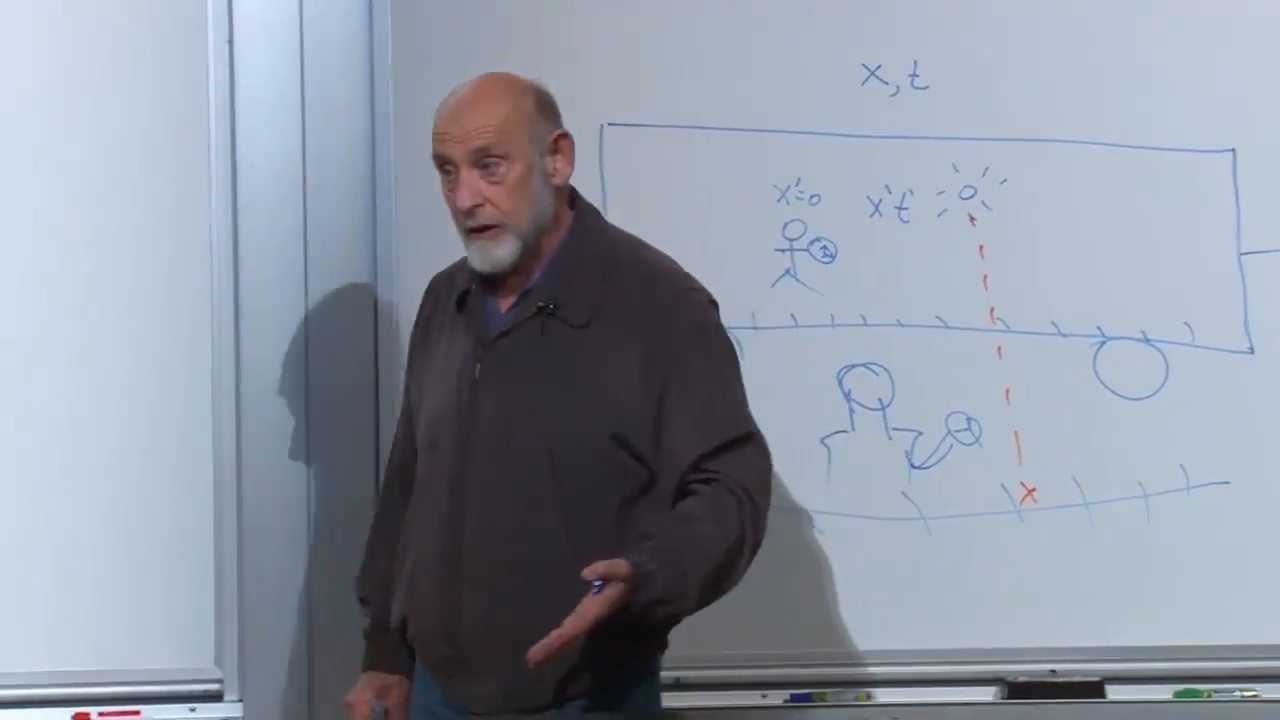
\includegraphics[width=0.90\textwidth]{lecture_02_figure_02.png}
\caption{Ánh xạ nghịch có cùng hệ số Lorentz và dấu trái ngược của vận tốc tương đối.}
\lectureframe{00:09:15}
\end{figure}

Đối với một phép boost dọc theo \(x\), các tọa độ ngang không đổi:
\begin{equation}
y'=y,
\qquad
z'=z.
\end{equation}

Có thể đọc ra tốc độ tương đối từ phương trình không gian mà không cần xét mẫu số của nó. Gốc tọa độ của đoàn tàu được xác định bởi \(x'=0\), và do đó
\begin{equation}
x'=0
\quad\Longleftrightarrow\quad
x-vt=0
\quad\Longleftrightarrow\quad
x=vt.
\label{eq:sr2-origin-worldline}
\end{equation}
Hệ số của \(t\) trong đường thế giới này là tốc độ của đoàn tàu trong các tọa độ của nhà ga.

\section{Ba hệ quy chiếu và sự hợp thành các phép boost}

Đặt một chiếc xe đồ chơi nhỏ cho trẻ em bên trong đoàn tàu. Đoàn tàu chuyển động với tốc độ \(v\) so với nhà ga, còn chiếc xe chuyển động dọc lối đi với tốc độ \(u\) so với hành khách trên tàu. Gọi tốc độ của chiếc xe so với nhà ga là \(w\). Trực giác Newton gợi ý \(w=u+v\), nhưng các phép biến đổi Lorentz mới là thứ phải quyết định.

Bây giờ có ba hệ tọa độ:
\begin{equation}
(x,t),\qquad (x',t'),\qquad (x'',t'').
\end{equation}
Hệ thứ nhất gắn với nhà ga, hệ thứ hai gắn với đoàn tàu, và hệ thứ ba gắn với chiếc xe. Giữa đoàn tàu và chiếc xe,
\begin{align}
x''&=\gamma_u(x'-ut'),&
t''&=\gamma_u(t'-ux'),
\label{eq:sr2-second-boost}\\
\gamma_u&=\frac{1}{\sqrt{1-u^2}}.
\end{align}

\begin{figure}[htbp]
\centering
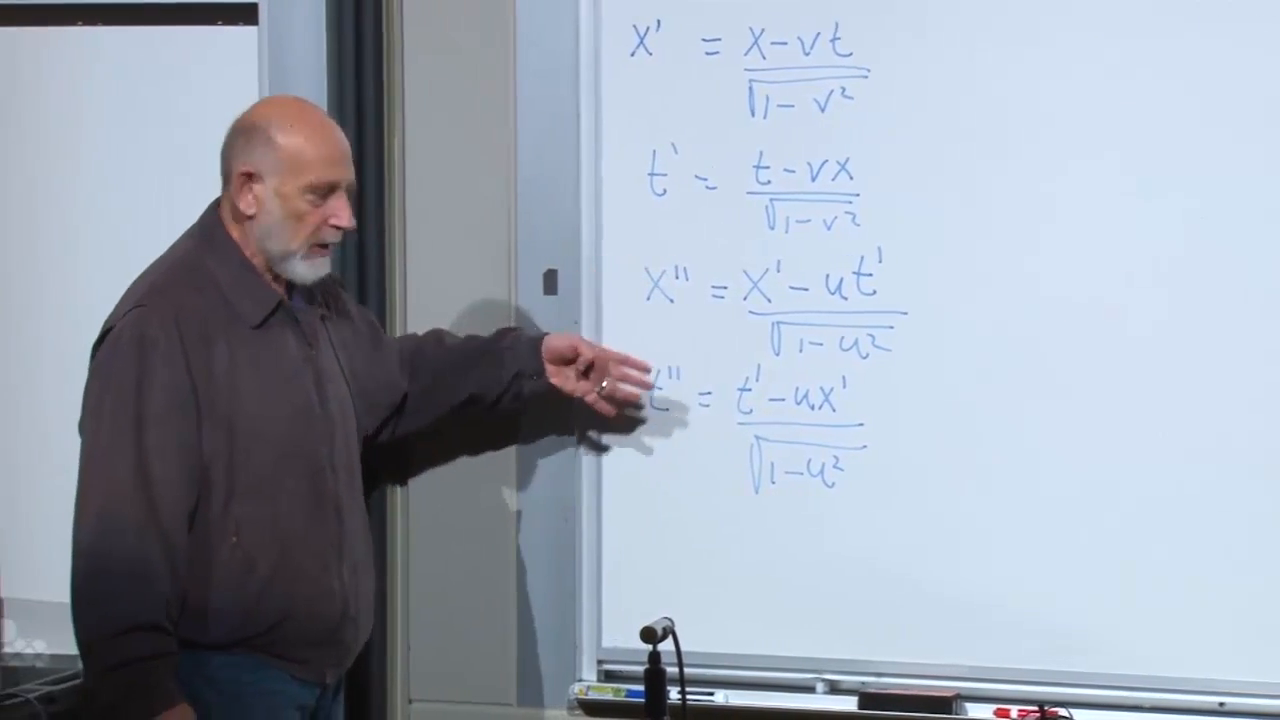
\includegraphics[width=0.90\textwidth]{lecture_02_figure_03.png}
\caption{Sau các công thức thuận từ nhà ga sang tàu là một phép biến đổi Lorentz thứ hai từ các tọa độ có phẩy sang các tọa độ hai phẩy.}
\lectureframe{00:14:55}
\end{figure}

\subsection{Thế một phép boost vào phép kia}

Phương trình không gian là đủ để tìm \(w\). Thế \eqref{eq:sr2-direct} vào phương trình thứ nhất của \eqref{eq:sr2-second-boost}:
\begin{align}
x''
&=\gamma_u(x'-ut')\\
&=\gamma_u\gamma_v\left[(x-vt)-u(t-vx)\right]\\
&=\gamma_u\gamma_v\left[(1+uv)x-(u+v)t\right].
\label{eq:sr2-composed-space}
\end{align}
Hai dấu trừ trong hạng \(uvx\) làm nó trở thành dương; hai hạng thời gian gộp lại thành \(-(u+v)t\).

\begin{figure}[htbp]
\centering
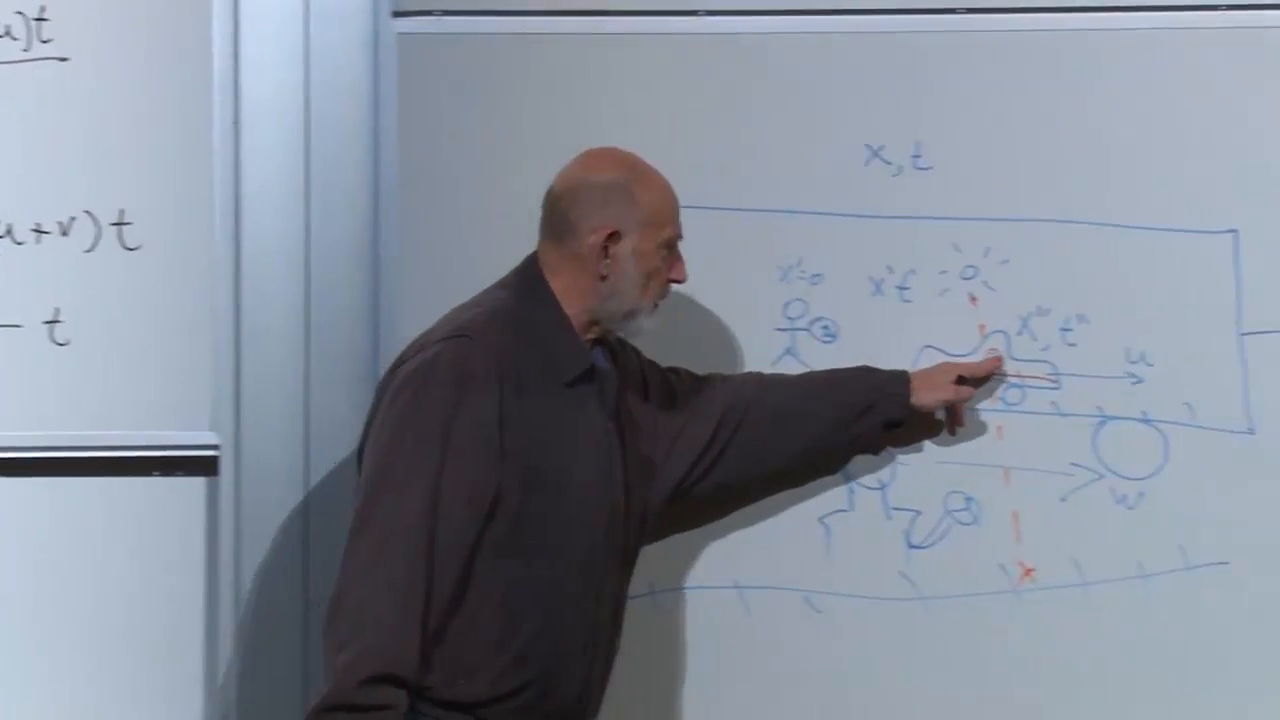
\includegraphics[width=0.91\textwidth]{lecture_02_figure_04.png}
\caption{Phép thế lồng nhau trước khi gom các hạng \(x\) và \(t\) trong phép boost hợp thành.}
\lectureframe{00:16:30}
\end{figure}

Như trước, mẫu số là không liên quan khi xác định gốc chuyển động. Chiếc xe đồ chơi đứng yên tại \(x''=0\), nên biểu thức trong ngoặc vuông ở \eqref{eq:sr2-composed-space} phải triệt tiêu:
\begin{equation}
(1+uv)x-(u+v)t=0.
\end{equation}
Vì thế, đường thế giới của nó trong hệ nhà ga là
\begin{equation}
x=\frac{u+v}{1+uv}\,t,
\end{equation}
và vận tốc của nó là
\begin{equation}
\boxed{w=\frac{u+v}{1+uv}}.
\label{eq:sr2-velocity-add-c1}
\end{equation}

\begin{figure}[htbp]
\centering
\includegraphics[width=0.91\textwidth]{lecture_02_figure_05.png}
\caption{Tử số sau khi đã gom hạng và đường thế giới \(x=[(u+v)/(1+uv)]t\) cho thấy vận tốc hợp thành.}
\lectureframe{00:19:30}
\end{figure}

Phương trình thời gian cũng hợp thành một cách nhất quán. Phép biến đổi đầy đủ từ nhà ga sang chiếc xe có dạng Lorentz
\begin{align}
x''&=\gamma_w(x-wt),&
t''&=\gamma_w(t-wx),
\end{align}
trong đó
\begin{equation}
\gamma_w=\frac{1}{\sqrt{1-w^2}}.
\end{equation}
Thật vậy,
\begin{equation}
\gamma_w=\gamma_u\gamma_v(1+uv),
\end{equation}
điều này suy ra bằng cách thế \eqref{eq:sr2-velocity-add-c1} rồi rút gọn. Do đó, hai phép boost cùng phương hợp thành một phép boost cùng phương khác.

\subsection{Khôi phục thứ nguyên}

\begin{classroomqa}
\audiencequestion{Vì sao mẫu số \(1+uv\) lại sai về mặt thứ nguyên trong các đơn vị thông thường?}
\lecturerresponse{Nó chỉ đúng vì \(c=1\) làm cho mọi vận tốc trở thành một tỷ phần không thứ nguyên của tốc độ ánh sáng. Trong các đơn vị quy ước, tích đó phải xuất hiện dưới dạng \(uv/c^2\), là một đại lượng không thứ nguyên. \lecturetimestamp{00:21:11}}
\end{classroomqa}

Công thức cộng vận tốc có thứ nguyên là
\begin{equation}
\boxed{
w=\frac{u+v}{1+\dfrac{uv}{c^2}}
}.
\label{eq:sr2-velocity-add}
\end{equation}

\begin{figure}[htbp]
\centering
\includegraphics[width=0.90\textwidth]{lecture_02_figure_06.png}
\caption{Tính nhất quán thứ nguyên khôi phục \(c^2\) dưới tích \(uv\).}
\lectureframe{00:22:06}
\end{figure}

Với \(\lvert u\rvert,\lvert v\rvert\ll c\),
\begin{equation}
\frac{uv}{c^2}\ll 1,
\end{equation}
nên
\begin{equation}
w\approx u+v.
\end{equation}
Phép cộng Newton là xấp xỉ tốc độ thấp chứ không phải một quy tắc riêng biệt.

\subsection{Hai miền số trị}

Trước hết lấy
\begin{equation}
u=v=0.01c.
\end{equation}
Trong đơn vị \(c=1\),
\begin{equation}
w=\frac{0.02}{1.0001}\approx 0.019998.
\end{equation}
Một phần trăm tốc độ ánh sáng đã vào khoảng \(3\times10^6\ {\rm m/s}\), nhưng hiệu chỉnh tương đối tính chỉ là một phần trên mười nghìn. Kết quả nhỏ hơn một chút so với giá trị Newton \(0.02c\).

\begin{figure}[htbp]
\centering
\includegraphics[width=0.90\textwidth]{lecture_02_figure_07.png}
\caption{Tại \(u=v=0.01c\), mẫu số chỉ khác 1 một lượng \(10^{-4}\).}
\lectureframe{00:24:23}
\end{figure}

Bây giờ lấy
\begin{equation}
u=v=0.9c.
\end{equation}
Newton sẽ dự đoán \(1.8c\). Thuyết tương đối cho
\begin{equation}
\frac{w}{c}
=\frac{0.9+0.9}{1+0.9^2}
=\frac{1.8}{1.81}
\approx 0.9945.
\label{eq:sr2-fast-example}
\end{equation}

\begin{figure}[htbp]
\centering
\includegraphics[width=0.90\textwidth]{lecture_02_figure_08.png}
\caption{Hai vận tốc bằng \(0.9c\) hợp thành \(1.8/1.81\), vẫn nhỏ hơn tốc độ ánh sáng.}
\lectureframe{00:25:48}
\end{figure}

Các phép boost liên tiếp với tốc độ dưới ánh sáng không thể vượt qua \(c\). Nếu \(u<c\) và \(v<c\), thì
\begin{equation}
1-\frac{w}{c}
=
\frac{\left(1-\frac{u}{c}\right)
      \left(1-\frac{v}{c}\right)}
     {1+\frac{uv}{c^2}}
>0.
\end{equation}
Mỗi phép boost bổ sung có thể đưa kết quả đến gần \(c\) hơn, nhưng không bao giờ vượt quá nó. Ở giá trị giới hạn \(u=c\),
\begin{equation}
w=\frac{c+v}{1+v/c}=c.
\end{equation}
Tốc độ ánh sáng là một điểm bất động của quy luật hợp thành.

\section{Phép đo tọa độ không phải là hình ảnh thị giác}

\begin{classroomqa}
\audiencequestion{Nếu đoàn tàu có các vách kính, liệu người quan sát ở nhà ga có thể chỉ cần nhìn cả hành khách lẫn chiếc xe đồ chơi cùng lúc rồi đọc trực tiếp chuyển động của chúng hay không?}
\lecturerresponse{Phép biến đổi Lorentz liên quan đến các phép đo tọa độ được thực hiện bằng những thước đo phân bố trong không gian và những đồng hồ đã được đồng bộ hóa. Một hình ảnh nhìn thấy còn chứa cả các thời gian truyền ánh sáng không bằng nhau từ những biến cố khác nhau tới người quan sát. Kính làm thay đổi quang cảnh nhìn thấy, chứ không làm thay đổi quan hệ tọa độ, và việc coi một hình ảnh như dữ liệu đồng thời sẽ đưa trở lại chính giả định về tính đồng thời mà thuyết tương đối đã sửa lại. \lecturetimestamp{00:27:53}}
\end{classroomqa}

Một biến cố có một vị trí và một thời điểm trong mỗi hệ, bất kể có ai tình cờ nhìn thấy nó đúng lúc ấy hay không. Hình ảnh quang học là một chủ đề hoàn toàn chính đáng, nhưng nó đòi hỏi một phép tính thứ hai để truy vết ánh sáng từ mỗi biến cố tới mắt. Bản thân các định luật biến đổi là phổ quát và không phụ thuộc vào các vách của đoàn tàu.

\section{Khoảng riêng trong ba chiều không gian}

Trở lại với hai biến cố, ban đầu một ở gốc tọa độ và biến cố kia ở \((x,t)\). Trong một chiều không gian,
\begin{equation}
\tau^2=t^2-x^2
\label{eq:sr2-interval-1d}
\end{equation}
trong đơn vị \(c=1\). Mọi hệ quán tính đều nhất trí rằng
\begin{equation}
\tau^2
=t^2-x^2
=t'^2-x'^2
=t''^2-x''^2.
\end{equation}
Các tọa độ thay đổi; khoảng riêng thì không.

Đối với một độ tách kiểu thời gian, một đồng hồ có thể chuyển động giữa hai biến cố. Nếu nó chỉ đúng ngọ ở biến cố thứ nhất, thì số chỉ đã trôi qua của nó ở biến cố thứ hai là thời gian riêng \(\tau\). Mệnh đề đó không phụ thuộc vào việc dùng hệ tọa độ nào để tính khoảng này.

\begin{figure}[htbp]
\centering
\includegraphics[width=0.90\textwidth]{lecture_02_figure_09.png}
\caption{Quan hệ thời gian riêng bất biến \(\tau^2=t^2-x^2\) được nhắc lại trước khi khôi phục các phương ngang.}
\lectureframe{00:30:18}
\end{figure}

\subsection{Các phép quay không gian khôi phục các phương ngang}

Hãy xét một phép quay thông thường của các trục không gian trước khi quay lại các phép boost. Một điểm không nằm trên trục \(x\) có bình phương khoảng cách không gian
\begin{equation}
r^2=x^2+y^2+z^2,
\end{equation}
đại lượng này bất biến dưới các phép quay theo định lý Pythagore thông thường. Vì thế khoảng không-thời gian trong \(3+1\) chiều là
\begin{equation}
\boxed{
\tau^2=t^2-x^2-y^2-z^2
}.
\label{eq:sr2-interval-3d}
\end{equation}
Khi khôi phục \(c\),
\begin{equation}
c^2\tau^2
=c^2t^2-x^2-y^2-z^2.
\end{equation}

\begin{figure}[htbp]
\centering
\includegraphics[width=0.90\textwidth]{lecture_02_figure_10.png}
\caption{Khoảng cách không gian Pythagore mở rộng đại lượng bất biến từ \(t^2-x^2\) thành \(t^2-x^2-y^2-z^2\).}
\lectureframe{00:34:23}
\end{figure}

Mọi tổ hợp của các phép quay không gian và các phép boost Lorentz đều bảo toàn \eqref{eq:sr2-interval-3d}. Các trục tọa độ thông thường có thể bất đồng về các thành phần nhưng nhất trí về khoảng cách Euclid; các hệ không-thời gian quán tính có thể bất đồng về các thành phần không gian và thời gian nhưng nhất trí về hiệu các bình phương này. Đại lượng bất biến đó là sự kiện hình học trung tâm của thuyết tương đối hẹp.

\begin{classroomqa}
\audiencequestion{Nếu hành khách thay chiếc xe đồ chơi bằng một chùm đèn pin chiếu về phía trước, thì người quan sát trên tàu và ở nhà ga có thu được cùng một tốc độ ánh sáng hay không?}
\lecturerresponse{Thay \(u=c\) vào \eqref{eq:sr2-velocity-add}. Khi đó \(w=(c+v)/(1+v/c)=c\). Trong đơn vị \(c=1\), tỷ số đơn giản là \((1+v)/(1+v)=1\). Cả hai hệ đều đo được cùng một tốc độ, đúng chính xác như yêu cầu. \lecturetimestamp{00:35:53}}
\end{classroomqa}

Vì thế, băn khoăn trước đó về các vách kính không phải là sự thất bại của tính bất biến của tốc độ ánh sáng. Đó là sự nhầm lẫn giữa một phép đo tọa độ và một hình ảnh thị giác bị trễ, rốt cuộc là một sự nhầm lẫn về tính đồng thời.

\section{Các tia null và nón ánh sáng}

Trong một chiều không gian, các tia sáng chuyển động sang phải và sang trái thỏa mãn
\begin{equation}
x=\pm t.
\end{equation}
Khoảng của chúng triệt tiêu:
\begin{equation}
t^2-x^2=0.
\end{equation}
Khác với khoảng cách Euclid, một khoảng không-thời gian bằng 0 không đòi hỏi các biến cố phải trùng nhau. Nó có nghĩa là một tín hiệu ánh sáng có thể nối chúng lại.

Khi khôi phục mọi phương không gian, một tia sáng tuân theo
\begin{equation}
t^2-x^2-y^2-z^2=0,
\label{eq:sr2-null}
\end{equation}
hoặc
\begin{equation}
r=t
\end{equation}
đối với ánh sáng hướng về tương lai trong đơn vị \(c=1\).

\begin{figure}[htbp]
\centering
\includegraphics[width=0.90\textwidth]{lecture_02_figure_11.png}
\caption{Ánh sáng theo bất kỳ phương không gian nào cũng đi theo một quỹ đạo null thỏa mãn \(t^2-(x^2+y^2+z^2)=0\).}
\lectureframe{00:39:28}
\end{figure}

Trong \(1+1\) chiều, tập null là một cặp đường thẳng \(45^\circ\). Với hai chiều không gian cộng thời gian, nó trở thành một hình nón; ba chiều không gian thì không thể biểu diễn đầy đủ trên bảng, nhưng phương trình xác định vẫn không đổi.

Nón ánh sáng tương lai gồm các biến cố mà ánh sáng phát ra tại gốc có thể tới được. Nón ánh sáng quá khứ gồm các biến cố mà từ đó ánh sáng có thể tới gốc. Cái này là cái kia lật ngược theo thời gian.

\begin{figure}[htbp]
\centering
\includegraphics[width=0.90\textwidth]{lecture_02_figure_12.png}
\caption{Các tia null \(45^\circ\) quét nên các nón ánh sáng tương lai và quá khứ trong một hình vẽ không-thời gian nhiều chiều hơn.}
\lectureframe{00:40:47}
\end{figure}

\begin{classroomqa}
\audiencequestion{Đại lượng bất biến tương ứng dưới các phép biến đổi Galileo trong cơ học Newton là gì?}
\lecturerresponse{Chính khoảng thời gian. Mọi người quan sát Newton đều nhất trí về \(\Delta t\), mặc dù họ bất đồng về độ dời không gian. Thuyết tương đối từ bỏ thời gian phổ quát và thay nó bằng khoảng không-thời gian bất biến. \lecturetimestamp{00:41:53}}
\end{classroomqa}

\section{Từ vectơ không gian đến bốn-vectơ}

Các vectơ ở đây là vectơ hình học, không phải vectơ trạng thái lượng tử. Một độ dời giữa hai điểm trong không gian thông thường có độ lớn và hướng. Có thể tịnh tiến gốc của nó về gốc tọa độ mà không làm thay đổi vectơ, và ba thành phần của nó có thể được ký hiệu là
\begin{equation}
x^i=(x^1,x^2,x^3)=(x,y,z),
\qquad i=1,2,3.
\end{equation}
Chỉ số Latin \(i\) chỉ chạy trên các phương không gian.

Một biến cố cần thêm một thành phần nữa, đó là thời gian của nó. Vì thế vị trí trong không-thời gian được viết là
\begin{equation}
x^\mu=(x^0,x^1,x^2,x^3)=(t,x,y,z),
\qquad \mu=0,1,2,3.
\label{eq:sr2-four-position}
\end{equation}
Theo quy ước lịch sử, thời gian là thành phần thứ không chứ không phải thứ tư:
\begin{equation}
x^0=t,\qquad x^1=x,\qquad x^2=y,\qquad x^3=z.
\end{equation}
Các chỉ số Hy Lạp như \(\mu\) chạy trên không-thời gian; các chỉ số Latin như \(i\) chạy trên không gian.

\begin{figure}[htbp]
\centering
\includegraphics[width=0.90\textwidth]{lecture_02_figure_13.png}
\caption{Các thành phần không gian \(x^i\) được mở rộng thành vị trí không-thời gian bốn thành phần \(x^\mu=(x^0,x^1,x^2,x^3)\).}
\lectureframe{00:46:05}
\end{figure}

Đại lượng bất biến trở thành
\begin{equation}
\tau^2
=(x^0)^2-(x^1)^2-(x^2)^2-(x^3)^2.
\end{equation}
Chỉ riêng ký hiệu này không bổ sung vật lý mới nào. Giá trị của nó là ở chỗ một phép biến đổi Lorentz tác dụng tuyến tính lên cả bốn thành phần, cũng như một phép quay tác dụng tuyến tính lên một vectơ không gian.

\begin{classroomqa}
\audiencequestion{Vì phép biến đổi là tuyến tính, liệu nó có thể được biểu diễn bằng một ma trận tác dụng lên một vectơ cột không?}
\lecturerresponse{Đúng. Với một phép boost theo \(x\), khối không tầm thường là \(\gamma_v\begin{pmatrix}1&-v\\-v&1\end{pmatrix}\) tác dụng lên \((t,x)^{\mathsf T}\), còn \(y\) và \(z\) thì không đổi. Ký hiệu ma trận là cách tự nhiên để hợp thành và sắp xếp các phép biến đổi Lorentz. \lecturetimestamp{00:48:14}}
\end{classroomqa}

Cụ thể,
\begin{equation}
\begin{pmatrix}
t'\\x'\\y'\\z'
\end{pmatrix}
=
\begin{pmatrix}
\gamma_v&-\gamma_v v&0&0\\
-\gamma_v v&\gamma_v&0&0\\
0&0&1&0\\
0&0&0&1
\end{pmatrix}
\begin{pmatrix}
t\\x\\y\\z
\end{pmatrix}.
\label{eq:sr2-boost-matrix}
\end{equation}

\section{Độ dời và bốn-vận tốc}

Xét sự chuyển từ vị trí của một sự kiện đến một đoạn ngắn trên đường thế giới của một hạt. Bốn-độ dời là
\begin{equation}
\Delta x^\mu
=(\Delta t,\Delta x,\Delta y,\Delta z).
\end{equation}
Khi một độ dời được gọi là nhỏ, tức là ta sắp dùng giải tích: \(\Delta x^\mu\) sẽ trở thành \(dx^\mu\). Tạm thời, ký hiệu hữu hạn làm cho hình học trở nên rõ ràng.

Độ tăng thời gian riêng dọc theo một đường thế giới loại thời thỏa mãn
\begin{equation}
(\Delta\tau)^2
=(\Delta t)^2-(\Delta x)^2-(\Delta y)^2-(\Delta z)^2.
\label{eq:sr2-proper-increment}
\end{equation}
Vận tốc thông thường lấy độ dời không gian chia cho thời gian tọa độ và có ba thành phần. Trái lại, bốn-vận tốc lấy bốn-độ dời chia cho thời gian riêng bất biến:
\begin{equation}
u^\mu
=\frac{\Delta x^\mu}{\Delta\tau}
\quad\longrightarrow\quad
\boxed{
u^\mu=\frac{dx^\mu}{d\tau}
}.
\label{eq:sr2-four-velocity}
\end{equation}

\begin{figure}[htbp]
\centering
\includegraphics[width=0.90\textwidth]{lecture_02_figure_14.png}
\caption{Một đoạn của đường thế giới xác định \(\Delta x^\mu\), đại lượng bất biến tương ứng \(\Delta\tau\), và bốn-vận tốc \(u^\mu=\Delta x^\mu/\Delta\tau\).}
\lectureframe{00:52:42}
\end{figure}

Đối tượng này có bốn thành phần và biến đổi như một bốn-vectơ. Quan hệ của nó với ba-vận tốc thông thường là câu hỏi tiếp theo, được cố ý để ngỏ ở đây. Việc giải quyết nó dẫn tới động lượng tương đối tính, năng lượng, gia tốc, và cuối cùng là sự khái quát hóa tương đối tính của \(F=ma\).
